\documentclass[journal=mamobx,manuscript=article]{achemso}


\usepackage[version=3]{mhchem} 
\usepackage{amsmath}
\usepackage{xcolor}
\usepackage{amsfonts}
\usepackage{amssymb}
\usepackage{graphicx}
\usepackage[english]{babel}
\usepackage{chemfig}
\newcommand{\species}[1]{\textit{#1} sp.}
\usepackage{subcaption}
\usepackage{cancel}



\newcommand{\leng}{\mathcal{L}}


%%%%%%%%%%%%%%%%%%%%%%%%%%%%%%%%%%%%%%%%%%%%%%%%%%%%%%%%%%%%%%%%%%%%%
%% If issues arise when submitting your manuscript, you may want to
%% un-comment the next line.  This provides information on the
%% version of every file you have used.
%%%%%%%%%%%%%%%%%%%%%%%%%%%%%%%%%%%%%%%%%%%%%%%%%%%%%%%%%%%%%%%%%%%%%
%%\listfiles


\newcommand*\mycommand[1]{\texttt{\emph{#1}}}
\SectionNumbersOn



\author{Sperydon Koumarianos}
\affiliation{Department of Physics and Astronomy, York University, Toronto, ON, Canada. M3J 1P3} 
\alsoaffiliation{Department of Mathematics and Statistics, York University, Toronto, ON, Canada.  M3J 1P3}

 
\author{Rohith Kaiyum}
\affiliation{Department of Physics and Astronomy, York University, Toronto, ON, Canada. M3J 1P3} 

\author{Christopher J. Barrett}
\affiliation{Department of Chemistry, McGill University, Montreal, QC, Canada.  H3A 2K6}
\alsoaffiliation{Department of Physics and Astronomy, York University, Toronto, ON, Canada. M3J 1P3} 

\author{Neal Madras}
\affiliation{Department of Mathematics and Statistics, York University, Toronto, ON, Canada.  M3J 1P3}

\author{Ozzy Mermut}
\affiliation{Department of Physics and Astronomy, York University, Toronto, ON, Canada. M3J 1P3}
\email{omermut@yorku.ca}



\title[An \textsf{achemso} demo]
  {Theory and Experiment of Chain Length Effects on the Adsorption of Polyelectrolytes onto Spherical Particles:  The Long and the Short of It --- Supporting Information }


\keywords{American Chemical Society, \LaTeX}

\begin{document}
\section{Calculations for the Mean-Field Lattice Model}

%\subsection{Setup of Mean-field lattice model}

%We shall use a lattice model to describe our experimental situation.  
%Lattices will appear in two ways:  (1) covering the surface of a sphere by a two-dimensional lattice, and
%(2) filling space with a regular three-dimensional lattice.  
%The geometry of the lattices will not play a significant role.
%We shall use the simple cubic lattice for our three-dimensional lattice.  
%We shall assume that the two-dimensional lattice has coordination number $q$ 
%(that is, each site on the surface has exactly $q$ neighbouring sites).  We assume that 
%the distance between lattice sites corresponds to the distance between adjacent monomers within a 
%polymer.  We assume that in equilibrium, every lattice site in the surface is covered by an adsorbed 
%monomer.  We also assume that in each polymer, either every 
%monomer is adsorbed or else no monomer is adsorbed.

%Our experiment has a large number $n_{sphere}$ of spheres in a solution of volume $V_{sol}$.  To simplify 
%our model and keep the concentrations the same, we shall consider only a single sphere in a solution
%of volume $V:=V_{sol}/n_{sphere}$.  We shall refer to this as our model system.
%We shall view this small three-dimensional region of the solution in our model system as being filled by a 
%cubic lattice.
%Let $V_{latt}$ be the number of lattice sites in our solution region of volume $V$. This is illustrated in the simple graphic in Figure 1.



%  \begin{figure}[H] 
%  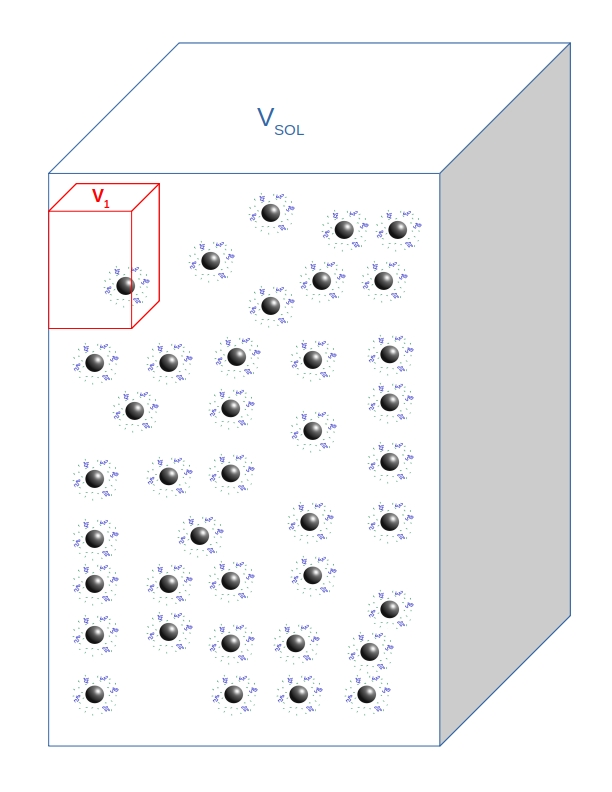
\includegraphics[scale=0.5]{fig7.jpg}
%\caption{Schematic of the model system (small box)
%inside the full solution (large box). The full system
%has volume $V_{sol}$ and contains many spheres.  The model
%system has volume $V$ and contains one sphere.}
%\label{figure 1}
%\end{figure}

\subsection{Estimating the Number of Configurations}

Here is a summary of the notation for the model system 
from Section 2.2 of the Main Paper.

Our model system has a single sphere in a solution of
volume $V$.  The model solution volume is filled by a 
simple cubic lattice, with the number of lattice sites in this volume denoted by $V_{latt}$.
The surface of the sphere is covered by a  two-dimensional lattice with coordination number $q$ 
(that is, each site on the surface has exactly $q$ neighbouring sites).  We assume that 
the distance between lattice sites corresponds to the distance between adjacent monomers within a 
polymer.  We assume that in equilibrium, every lattice site in the surface is covered by an adsorbed 
monomer.  We also assume that in each polymer, either every 
monomer is adsorbed or else no monomer is adsorbed.
 



We assume that our model system has $n_L$ ``long'' chains, each
with $\leng_L$ monomers, as well as $n_S$ ``short''
chains, each with $\leng_S$ monomers.

We define $n=\leng_L/\leng_S$, so that $\leng_L=n\leng_S$.   To make the total mass
of the two sizes of polymers the same, we can
declare $n_S=n \cdot n_L$, but we will not use
this relation.  It will suffice that $n_S$ and 
$n\cdot n_L$ have similar orders of magnitude.

We let $S_{latt}$ be the number of lattice sites on 
the surface of one sphere.  Then the maximum number of 
long chains that can adsorb onto the surface is 
$S_{latt}/\leng_S$, which we call $a$. For 
simplicity, we assume that $a$ is an integer.

%We shall consider polymers of two different lengths, which we shall call ``short'' and ``long.''  Their lengths
%will be described by two positive integer parameters $W$ and $n$.

%\begin{verse}
%A \textbf{short polymer} will consist of $W$ monomers.  
%Let $n_S$ be the number of short polymers in the model system. 
%\\
%A \textbf{long polymer} will consist of $nW$ monomers.  
%Let $n_L$ be the number of long polymers in the model system. 
%\end{verse}
%We shall often refer to our short and long polymers as $W$-mers and $nW$-mers respectively.
%We shall want the total mass of the two kinds of monomers in our system to be the same, so we 
%shall assume that $n_S \,=\, n\cdot n_L$.

%Let $A_{latt}$ be the number of lattice sites on the surface of one sphere, and let $a$
%be the number of long polymers that would exactly cover all the sites of the surface:
%\[    a  \;=\;  \frac{A_{latt}}{nW}   \,  .  \]
%Then $na$ is the number of short polymers that can completely cover the surface.
%For simplicity, we assume that $a$ is an integer.

%We shall see that the underlying entropic reason that
%mostly long chains get adsorbed is that $V_{latt}\gg A_{latt}$, i.e.\ there are many more possible locations in 
%the three-dimensional solution than on the two-dimensional surface.


%We shall model our polymer configurations in the solution in a slightly different way from those on the surface.
%The difference in approach is due to the fact that the polymers are dense on the surface but 
%dilute in the solution.  We shall model the polymer configurations in the solution as a collection of 
%self-avoiding walks in the cubic lattice, with no interaction between walks (because of the dilute solution).
%For the polymers adsorbed densely on the surface lattice, we shall use mean-field calculations 
%of the Flory-Huggins type 
% (similar to the lattice approach in Park et al., Macromolecules 2001;
%(see also Section XII.1 of Flory\cite{Flory1953}).

% Recall that our ensemble consists of $n_S$ (short) $W$-mers and $n_L$ (long) $nW$-mers.
%Of these, some are adsorbed onto the surface of the sphere, and the others float freely in the 
%solution of volume $V_1$.  

We write $\mathcal{E}_j$ for the set of all configurations (of $n_L$ long chains and $n_S$ short chains) that have exactly $j$ 
$\leng_L$-mers adsorbed onto the surface.  
The possible values of $j$ are the integers from 0 to $a$.
For each configuration in $\mathcal{E}_j$, it must be true that:
%We let $j$ denote the number of (long) $\leng_L$-mers that are adsorbed 
%onto the surface in a particular configuration of the model system.  This implies that
%\begin{verse}
\\
 ($i$) the number of $\leng_L$-mers in solution is $n_L-j$;
 \\
 ($ii$) the number of $\leng_S$-mers adsorbed onto the surface is $n(a-j)$; and 
%(because there are $anW$ sites on the
% surface, all occupied, of which $jnW$ are occupied by $nW$-mers, leaving $anW-jnW$ to be 
% occupied by $W$-mers); and
 \\
 ($iii$) the number of $\leng_L$-mers in solution is $n_S-n(a-j)$.
% \end{verse}  
\\
The full space of configurations in our model is $\cup_{j=0}^a {\mathcal{E}_j}$, 
which we call $\mathcal{E}$.

%Since the only energy in this model comes from the adsorption contacts between monomer and surface,
%and since the number of such contacts is the same (namely $S_{latt}$) in every configuration
%in $\mathcal{E}$, we see that 
Since the energy of every configuration of $\mathcal{E}$ is exactly the same,
%Therefore, according to the Boltzmann distribution, \textit{every configuration in $\mathcal{E}$ is equally likely}.  Thus
the calculation of probabilities of events is equivalent to counting the configurations.
In particular, writing $|\mathcal{A}|$ for the number of configurations in a set $\mathcal{A}$, we have
\[
    \hbox{Probability that $j$ long polymers are adsorbed}  \;=\; 
    \frac{|\mathcal{E}_j|}{|\mathcal{E}|}\,,   \hspace{5mm}(j=0,1,\ldots,a).
\]
Thus, to find the most likely number of $\leng_L$-mers (and $\leng_S$-mers) to be adsorbed onto the sphere,
we need to find which of the sets $\mathcal{E}_j$ is largest.


In order to better comprehend the model we provide an illustration Figure \ref{figure 2supp} with much simpler values than what would be considered standard chain lengths in polymer science. We let each lattice point of area of one mer of PAA, be a square on the grid. 
%Additionally, each long chain mer contact is represented by an L and a short chain mer by an S on the grid.  
Suppose a short chain is %30-mers and long chain is 90-mers and the colloid surface has 3000 available single mer sites.
25-mers and long chain is 75-mers and the colloid surface has 2025 available single mer sites.
In the parameters of this model, we have 
$S_{latt}=2025$, $\leng_S=25$,
$\leng_L=75$,$n=3$, and $a=2025/75=27$.
For simplicity, the figure shows each short chain
fills a $5\times 5$ square of lattice points, and each
long chain fills three adjacent $5\times 5$ squares.
We can think of the model initially with the colloid surface sites fully covered exclusively by short chains, which in this concrete example requires 81 short chains (a). We then remove 3 short chains and replace them with our first long chain (b). 
We can think of continuing this process of adding more and more long chains in place of the equivalent number of mers in short chains (c,d,e) until we reach the maximum number of long chains (f).
%value for $\mathcal{E}_{j}$.

\begin{figure}[H]
    \begin{subfigure}[b]{0.4\textwidth}
        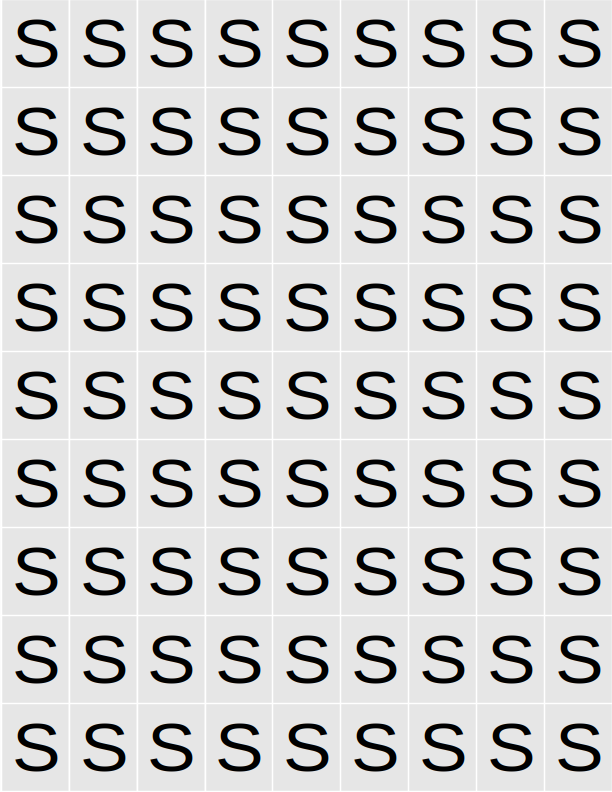
\includegraphics[scale=0.15]{fig8a.png}
        \caption{ $\mathcal{E}_0$:  0 long \& 81 short \\chains on Colloid Surface}
        \label{fig:A}
    \end{subfigure}
    \begin{subfigure}[b]{0.4\textwidth}
        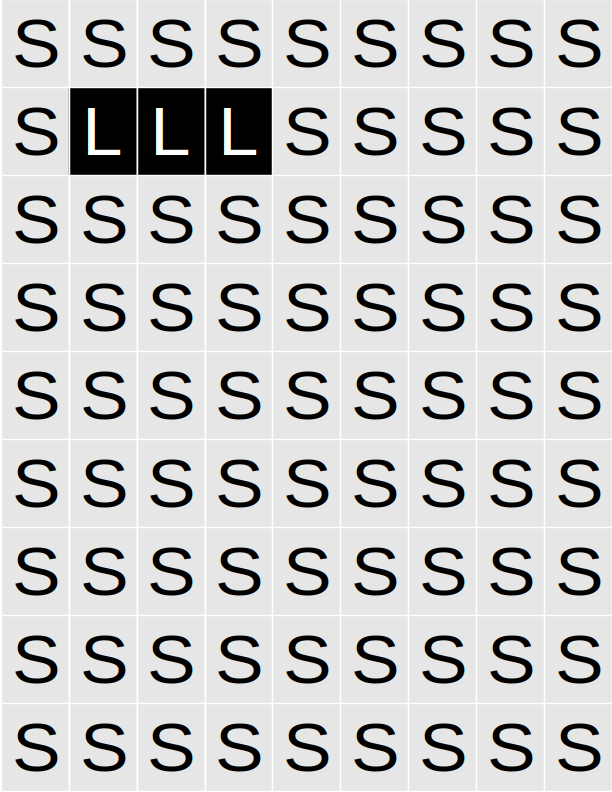
\includegraphics[scale=0.15]{fig8b.png}
        \caption{$\mathcal{E}_1$: 1 long \& 78 short \\chains on Colloid Surface}
        \label{fig:B}
    \end{subfigure}
    \begin{subfigure}[b]{0.4\textwidth}
        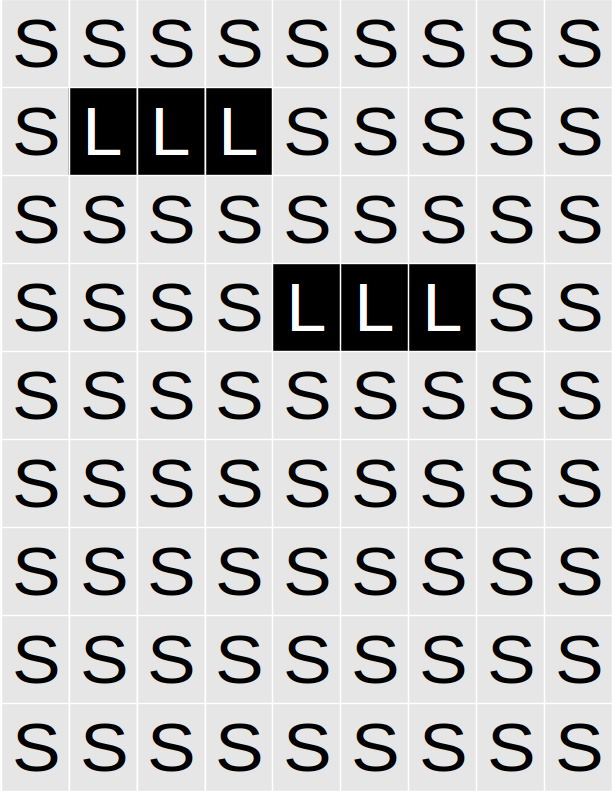
\includegraphics[scale=0.15]{fig8c.png}
        \caption{$\mathcal{E}_2$: 2 long \& 75 short \\chains on Colloid Surface}
        \label{fig:C}
    \end{subfigure}
    \begin{subfigure}[b]{0.4\textwidth}
        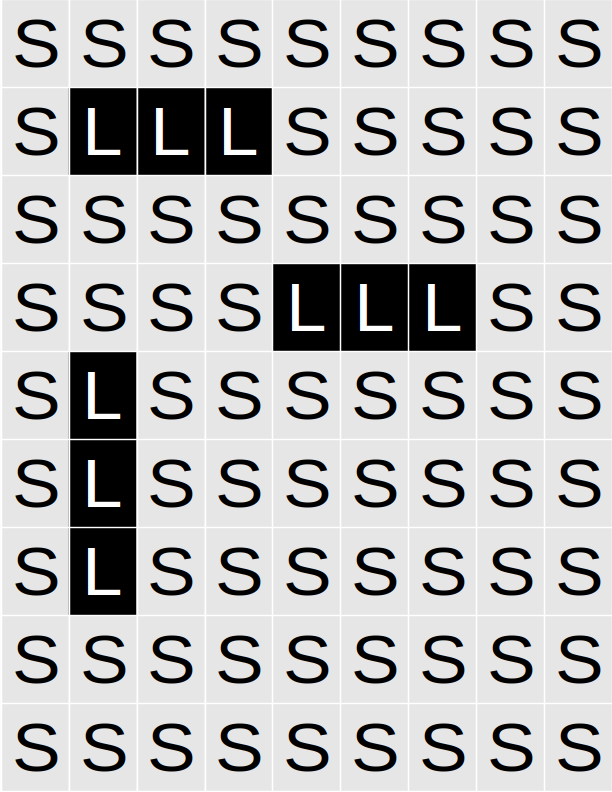
\includegraphics[scale=0.15]{fig8d.png}
        \caption{$\mathcal{E}_3$:  3 long \& 72 short \\chains on Colloid Surface}
        \label{fig:D}
    \end{subfigure}
    \begin{subfigure}[b]{0.4\textwidth}
        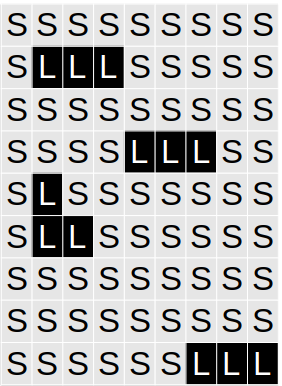
\includegraphics[scale=0.315]{rightangleL.png}
        \caption{$\mathcal{E}_4$:  4 long \& 69 short \\chains on Colloid Surface}
        \label{fig:E}
    \end{subfigure}
    \begin{subfigure}[b]{0.4\textwidth}
        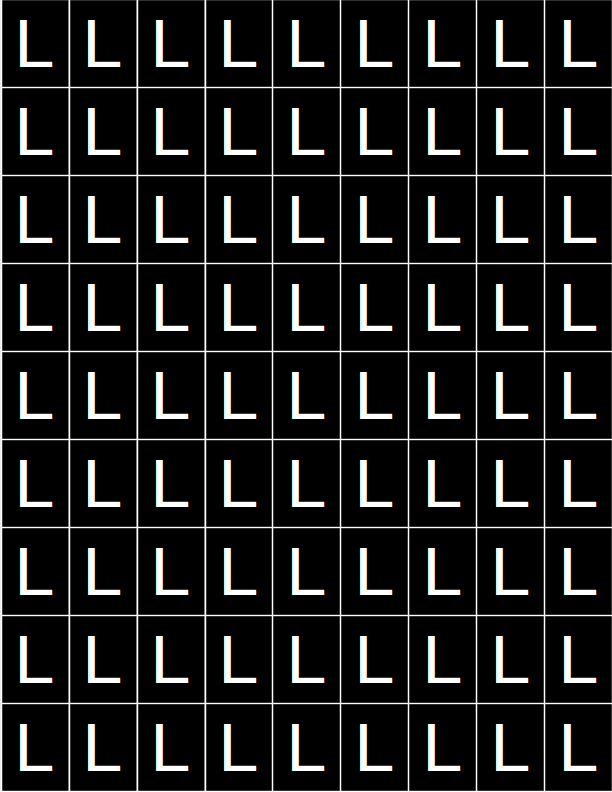
\includegraphics[scale=0.15]{fig8f.png}
        \caption{$\mathcal{E}_{27}$:  27 long \& 0 short \\ chains on Colloid Surface}
        \label{fig:F}
    \end{subfigure}
    \caption{Schematic of configurations in 
    $\mathcal{E}_j$ for $j=0,1,2,3,4,27$, with
    $j$ long chains and $81-3j$ short chains adsorbed
    onto the colloid surface.  Each S represents a $5\times 5$ square of lattice points covered by one short chain; similarly, three contiguous L's are covered by one long chain. 
    }
    %Process of Sampling Full Surface Coverage Combinations of ever increasing long chains that are substituting multiple short chains  on Colloid}
    \label{figure 2supp}
\end{figure}



% \noindent We now proceed to estimate the size of each $\mathcal{E}_j$.

\smallskip

%The configuration of a single  polymer in a dilute solution is often modeled by
%a self-avoiding walk (SAW) in a lattice, i.e.\  a path in the lattice that does not visit any site more than once.
%A fundamental property of SAWs is the following.  
%Let $c_{\ell}$ be
%the number of SAWs that start from a specified lattice site (``the origin'') and visit a total of $\ell$ sites
%(including the starting site).   Then the 
%asymptotic behaviour of $c_{\ell}$ on the three-dimensional cubic lattice is 
%\begin{equation}
%    \label{eq.sawscale}
%       c_{\ell}  \;\sim  \;  A_3 \, {\ell}^{\gamma_3-1}  \mu_3^{\ell}    \hspace{5mm}\hbox{as $\ell\rightarrow\infty$}.
%\end{equation}
%% (This has not been proven rigorously, but even mathematicians do not doubt its truth.) 
%Here $\mu_3$ and $A_3$ depend on the choice of lattice, but $\gamma_3$ is a universal critical exponent
%that is the same for all three-dimensional lattices.  
%Their values are known to be approximately \cite{Chen2002,Madras2013}
%\begin{equation}
%   \label{eq.gammas}   \mu_3 \;=\;  4.684, \hspace{5mm}
 %       \gamma_3 \;=\;  1.162,    \hspace{5mm}\hbox{and}\hspace{5mm}
%    A_3  \;=\;    0.2573  \,.  %1.205/4.683 \;=\;  \,.
%\end{equation}
%(Estimation in \cite{Chen2002} is for the 
%number of SAWs with $\ell$ \textit{steps} (i.e.\ $\ell+1$ \textit{sites}), which we write  $c_{\ell+1}=(A_3\mu_3)\ell^{\gamma_3-1}\mu_3^{\ell}$; reference \cite{Chen2002} obtains $A_3\mu_3=1.205$.)

%Since the number of sites in the lattice corresponding to the region of solution is $V_{latt}$, 
%we have $V_{latt}c_{\ell}$ ways to place a polymer of size ${\ell}$.  As we are neglecting the
%possibility of overlapping polymers in the dilute solution, it follows that the number of ways to 
%place $N$ identical $\ell$-mers is 
%\begin{equation}
%  \label{eq.Npoly}
%   \frac{(V_{latt}c_{\ell})^N}{N!}  \,.   
%\end{equation}

%\smallskip

In the Main Paper, we found that the number of configurations in $\mathcal{E}_j$ is
\begin{equation}
    |\mathcal{E}_j|  
      \; = \; \frac{ \Psi_L^{n_L-j} }{(n_L-j)!} \,
          \frac{ \Psi_S^{n_S-n(a-j)} }{(n_S-n(a-j))!} \,  G(j)
%           \frac{\tilde{w}_1\tilde{w}_2\cdots \tilde{w}_j}{j!}
 %                    \,   \frac{\tilde{u}_{nj+1}\tilde{u}_{nj+2}\cdots \tilde{u}_{an}}{(n(a-j))!}
        \label{eq.Yjsupp}
\end{equation}
where 
\begin{equation}
    \label{eq.psidefsupp}   
   \Psi_L\;=\;V_{latt} A_3 (\leng_L)^{\gamma_3-1} \mu_{3}^{\leng_L} \,,  
    \hspace{5mm} %\hbox{and} \hspace{5mm}
     \Psi_S \;=\; V_{latt}A_3{\leng_S}^{\gamma_3-1}\mu_3^{\leng_S} \,,
\end{equation}
and $G(j)$ is the number of ways to cover the surface
with $j$ $\leng_L$-mers and $n(a-j)$ $\leng_S$-mers.
(Here $A_3$, $\gamma_3$, and $\mu_3$ are constants 
related to self-avoiding walks.)  
Computing $G(j)$ is a hard combinatorial problem, so we shall use a mean-field approximation of the Flory-Huggins type, which we now explain 
% (similar to the lattice approach in Park et al., Macromolecules 2001;
(see also Section XII.1 of P.J. Flory, \textit{Principles of Polymer Chemistry}, Cornell University Press, 1953).
%\cite{Flory1953}),


For a particular choice of $j$, we want to know the number of ways to place $j$ $\leng_L$-mers 
and $a(n-j)$ $\leng_S$-mers on the surface,
without overlapping.  %, to fill all % $anW$ 
%the lattice sites on the sphere's surface.
We shall place one polymer at a time, starting with the long ones.
Let $\tilde{w}_k$ be the number of ways to place the $k^{th}$ $\leng_L$-mer on the surface, given that
$(k-1)$ $\leng_L$-mers have already been placed.  
To begin with, there are $a\leng_L-(k-1)\leng_L$ available sites for the first monomer.  Recall that  $q$ is the number of
neighbours of each site in the surface lattice.
In the absence of other polymers, there would be $q$ choices for the second monomer in the chain,
and $q-1$ choices for each monomer after that (here we are using the non-reversed walk model of a polymer
instead of the fully self-avoiding model).  But the number of choices should on average be reduced 
by the fraction of the surface that has already been covered.  
Thus, when we are trying to place the second monomer of our chain, there are
$a\leng_L-(k-1)\leng_L-1$ unoccupied sites, so each site has 
probability $[a\leng_L-(k-1)\leng_L-1]/[a\leng_L]$ of being available.  
Thus there are $q[a\leng_L-(k-1)\leng_L-1]/[a\leng_L]$ choices for the second monomer.  
Similarly, after $i$ monomers of the current chain have been placed ($i\geq 2$), the fraction of the
surface that has not been covered is $[a\leng_L-(k-1)\leng_L-i]/[a\leng_L]$, so there are 
$(q-1)[a\leng_L-(k-1)\leng_L-i]/[a\leng_L]$ choices for the $(i+1)^{th}$ monomer in this chain.  
We conclude that 
\begin{eqnarray}
   \tilde{w}_k  & = &   [a\leng_L-(k-1)\leng_L]\,\times \,q\left(\frac{ a\leng_L-(k-1)\leng_L-1}{a\leng_L}\right)    \,\times
   \nonumber    \\
   & &    \hspace{22mm}
     \prod_{i=2}^{\leng_L-1}(q-1)\left(\frac{ a\leng_L-(k-1)\leng_L-i}{a\leng_L}\right)  
      \nonumber \\
 & = &    \frac{[a\leng_L-(k-1)\leng_L]!}{[a\leng_L-k\leng_L]!} \,q\,  \frac{(q-1)^{\leng_L-2}}{(a\leng_L)^{\leng_L-1}}  
     \nonumber    \\
     & = &    \frac{[a\leng_L-(k-1)\leng_L]!}{[a\leng_L-k\leng_L]!}   a\leng_L \frac{q}{(q-1)^2}\left(  \frac{q-1}{a\leng_L}\right)^{\leng_L}.
     \label{eq.wk2supp}
\end{eqnarray}
Similarly, let $\tilde{u}_{\ell}$ be the number of ways to place the $\ell^{th}$ $\leng_S$-mer on the surface, given that
${\ell}-1$ $\leng_S$-mers (or a total of $(\ell-1)\leng_S$ monomers) have already been placed.   The same 
argument as for $\tilde{w}_k$ gives
\begin{eqnarray}
   \tilde{u}_{\ell}  
 & = &    \frac{[an\leng_S-(\ell-1)\leng_S]!}{[an\leng_S-\ell \leng_S]!} \,q\,  \frac{(q-1)^{\leng_S-2}}{(an\leng_S)^{\leng_S-1}}  
     \nonumber    \\
     & = &    \frac{[an\leng_S-(\ell-1)\leng_S]!}{[an\leng_S-\ell \leng_S]!}   an\leng_S \frac{q}{(q-1)^2}\left(  \frac{q-1}{an\leng_S}\right)^{\leng_S}.
     \label{eq.uell2supp}
\end{eqnarray}
We can now express the combinatorial quantity $G(j)$ 
in Equation (\ref{eq.Yjsupp}) as
\begin{equation}
    \label{eq.Gformulasupp}
      G(j) \;=\;      \frac{\tilde{w}_1\tilde{w}_2\cdots \tilde{w}_j}{j!}
                    \,   \frac{\tilde{u}_{nj+1}\tilde{u}_{nj+2}\cdots \tilde{u}_{an}}{(n(a-j))!}  \,.
\end{equation}



%To evaluate $|\mathcal{E}_j|$, we assume that the solution of unadsorbed polymers 
%is dilute enough that we don't need to worry about mutual exclusion between the free floating polymers.   
%For $\mathcal{E}_j$, we have $j$ adsorbed $nW$-mers, $na-nj$ adsorbed $W$-mers, 
%$n_L-j$ desorbed $nW$-mers, and $n_S-n(a-j)$ desorbed $W$-mers.   Thus, recalling 
%Equations (\ref{eq.sawscale}) and  (\ref{eq.Npoly}), we have
%\begin{equation}
%    |\mathcal{E}_j|  
%      \; = \; \frac{ \Psi_L^{n_L-j} }{(n_L-j)!} \,
%          \frac{ \Psi_S^{n_S-n(a-j)} }{(n_S-n(a-j))!} \,
%           \frac{\tilde{w}_1\tilde{w}_2\cdots \tilde{w}_j}{j!}
%                     \,   \frac{\tilde{u}_{nj+1}\tilde{u}_{nj+2}\cdots \tilde{u}_{an}}{(n(a-j))!}
%                                  \nonumber   \\
%            & & \hspace{7mm}  \times \, \frac{\tilde{w}_1\tilde{w}_2\cdots \tilde{w}_j}{j!}
%                     \,   \frac{\tilde{u}_{nj+1}\tilde{u}_{nj+2}\cdots \tilde{u}_{an}}{(n(a-j))!}  % \,e^{-nW\epsilon/kT}
%        \label{eq.Yj}
%\end{equation}
%where 
%\begin{equation}
%    \label{eq.psidef}   
%   \Psi_L\;=\;V_{latt} A_3 (nW)^{\gamma_3-1} \mu_{3}^{nW}   
%    \hspace{5mm}\hbox{and} \hspace{5mm}
%     \Psi_S \;=\; V_{latt}A_3W^{\gamma_3-1}\mu_3^W \,.
%\end{equation}




To determine which value of $j$ maximizes $|\mathcal{E}_j|$, we look at ratios of consecutive terms, using Equations (\ref{eq.Yjsupp}--\ref{eq.Gformulasupp}):
\begin{eqnarray}
    \frac{|\mathcal{E}_{j+1}|}{|\mathcal{E}_j|}   & = & 
 \frac{
     \left(\frac{\Psi_L^{n_{L}-j-1}}{(n_L-j-1)!}\right)\cdot\left(\frac{\Psi_S^{n_S-n(a-j-1)}}{
    (n_S-n(a-j-1))!}\right) 
      }{
 \left(\frac{\Psi_L^{n_{L}-j}}{(n_L-j)!}\right)\cdot\left(\frac{\Psi_S^{n_S-n(a-j)}}{
    (n_S-n(a-j))!}\right)  }  \,   \frac{\tilde{w}_{j+1} }{  \tilde{u}_{nj+1}\cdots \tilde{u}_{n(j+1)} } 
    \nonumber \\
    & & \hspace{42mm}  
     \times   \, \frac{ j! \, (na-nj)!}{(j+1)!\, (na-nj-n)!}  
    \nonumber    \\
    & = & \frac{\Psi_S^n}{\Psi_L}
   % \frac{ \left(  V_{latt} A_3 W^{\gamma_3-1}\right)^{n-1}}{n^{\gamma_3-1}}
    \,   \frac{\tilde{w}_{j+1} }{  \tilde{u}_{nj+1}\cdots \tilde{u}_{n(j+1)} }   \,\left(  \frac{n_L-j}{j+1}\right)
    \nonumber \\
    & &   \hspace{8mm}  \times \;  \frac{(na-nj)\cdots (na-nj-n+1)}{(n_S-na+nj+1)\cdots(n_S-na+nj+n)} \,.
        \label{eq.Yratio1supp}
\end{eqnarray}
From now on, we replace $\leng_L$ by $n\leng_S$.
By Equation (\ref{eq.psidefsupp}), we have
\begin{equation}
   \label{eq.psiratiosupp} 
      \frac{\Psi_S^n}{\Psi_L}   \;=\;   \frac{ (V_{latt}\, A_3 \,\leng_S^{\gamma_3-1})^{n-1}}{n^{\gamma_3-1}}\,.
\end{equation}
From Equations (\ref{eq.wk2supp}) and (\ref{eq.uell2supp}), we find
\begin{eqnarray}
     \frac{\tilde{w}_{j+1} }{  \tilde{u}_{nj+1}\cdots \tilde{u}_{n(j+1)} }  & = & 
        \left( \frac{(q-1)^2}{qan\leng_S}\right)^{n-1}   \times \,
    \frac{   \frac{(an\leng_S-jn\leng_S)!}{(an\leng_S-(j+1)n\leng_S)!}  }{
        \prod_{\ell=0}^{n-1} \frac{ (an\leng_S-(nj+\ell)\leng_S)!}{(an\leng_S-(nj+\ell+1)\leng_S)!}   }
     \nonumber  \\
     & = & \left( \frac{(q-1)^2}{qan\leng_S}\right)^{n-1}  \,\times\, 1.
     \label{eq.Yratioasupp}     
\end{eqnarray}
Next we use the approximation   $(c+1)(c+2)\cdots (c+m) \,\approx \,(c+\frac{m}{2})^m$
(essentially, replacing the geometric mean by the arithmetic mean) to obtain
\begin{equation}
       \frac{(na-nj)\cdots (na-nj-n+1)}{(n_S-na+nj+1)\cdots(n_S-na+nj+n)} 
       \; \approx \;    \frac{ [na-(j+\frac{1}{2})n]^n }{ [n_S-na+nj+\frac{n}{2}]^n} \,.\hspace{3mm}
  %     \nonumber  \\
  %     & \approx & \left(  \frac{n(a-j-\frac{1}{2})}{n_S-(a-j-\frac{1}{2})}\right)^n  .
      \label{eq.Yratiobsupp}
\end{equation} 
Now, putting Equations (\ref{eq.psiratiosupp}--\ref{eq.Yratiobsupp}) back into (\ref{eq.Yratio1supp}), we obtain
\begin{equation}
    \label{eq.Yratio2supp}
       \frac{|\mathcal{E}_{j+1}|}{|\mathcal{E}_j|} \; \approx \; 
       \left( h(j)\right)^{n+o(n)},
       \hspace{5mm}\hbox{where}\hspace{5mm}
       h(j)  \;=\;
       \frac{V_{latt}A_3\leng_S^{\gamma_3-1}(q-1)^2}{aq\leng_S} \,
          \frac{(a-j-\frac{1}{2})}{n_S-n(a-j-\frac{1}{2})}  \,.
\end{equation}
%The quantity on the right of Equation (\ref{eq.Yratio2}) decreases in $j$.  
Let $j^*$ be the 
smallest value of $j$ for which $h(j)$ is less than 1.
%Then we see that $|\mathcal{E}_{j+1}|/|\mathcal{E}_j|<1$ whenever $j\geq j^*$, and 
%$|\mathcal{E}_{j+1}|/|\mathcal{E}_j|\geq 1$ whenever $j< j^*$.
%That is, $|\mathcal{E}_j|$ is decreasing in $j$ when $j\geq j^*$, and 
%increasing when $j< j^*$.
%It follows that $|\mathcal{E}_j|$ is maximized at $j=j^*$, and that we can find $j^*$ by seeing 
%where the right-hand side of Equation (\ref{eq.Yratio2}) is close to 1.   Thus $j^*$ satisfies
As explained in the main paper, the quantity $|\mathcal{E}_j|$
is maximized at $j=j^*$, and $j^*$ satisfies 
$h(j^*)\approx 1$, which is equivalent to
\[     1  \;\approx \; 
     K  \,%\frac{ V_{latt}A_3W^{\gamma_3-1}(q-1)^2}{aWq} \,
          \frac{a-j^*-\frac{1}{2}}{n_S-n(a-j^*-\frac{1}{2})}    \,,  
             \hspace{5mm}\hbox{where}\hspace{5mm}
             K \;=\;   \frac{ V_{latt} }{a\leng_S}\, \frac{   A_3\leng_S^{\gamma_3-1}(q-1)^2}{q} \,.
\]
The above approximation can be rewritten as 
\[       a-j^*-\frac{1}{2} \; \approx\;    \frac{n_S}{K+n}   \,.
\]
We observe that $K\gg n$; indeed,  $V_{latt}/a\leng_S n \,=\,V_{latt}/S_{latt}\gg 1$.  
Thus we can replace $K+n$ by $K$ in the above, and omit the small term $\frac{1}{2}$, resulting in the   
approximation 
\begin{equation}
    \label{eq.jstarsupp}
     1-\frac{j^*}{a}     \; \approx   \; 
        \left(  \frac{n_S\,\leng_S}{V_{latt} }\right) \,\left(   \frac{q}{A_3\leng_S^{\gamma_3-1}(q-1)^2}\right)  \,.
\end{equation}
%The above equation can be interpreted as follows.  The left hand side, $1-j^*/a$, is the fraction of the
%sphere's surface that is covered by short monomers.  
%The quantity in the second set of 
%parentheses in Equation (\ref{eq.jstar}) cannot be large, since $q<(q-1)^2$ and $\gamma_3>1$.
%The ratio $n_S\leng_S/V_{latt}$ gives
%the concentration of monomers corresponding to those appearing on the short chains only.
%If the solution is fairly dilute, then we see that the right (and hence the left) side of (\ref{eq.jstar}) is small,
%and therefore only a small fraction of the surface is covered by short polymers.
See the Main Paper for the discussion and interpretation of Equation (\ref{eq.jstarsupp}).

[\textit{Remark:}  It is interesting to observe that $n_L$ does not appear in Equation (\ref{eq.jstarsupp}).  
In the expression for $|\mathcal{E}_{j+1}|/|\mathcal{E}_j|$,   only $n_S$ appears inside the 
expression that is raised to the power $n$, while $n_L$ appears outside this expression and is
raised to the power 1.]  

\subsection{Interpretations about $|\mathcal{E}_{j}|$ from ratio $\frac{|\mathcal{E}_{j+1}|}{|\mathcal{E}_{j}}|$}



Figure \ref{figure 9} graphically portrays 
that as one increases the number of long chains in a scenario of full surface coverage of the colloid, the ratio of probabilities decreases and 
eventually crosses the threshold of 
%the functional value 
being equal to one ($\frac{|\mathcal{E}_{j+1}|}{|\mathcal{E}_{j}|}=1$). 
This threshold is representative of two consecutive configurations being equal in value and thus the the divided differences of $|\mathcal{E}_{j+1}|$ and $|\mathcal{E}_{j}|$ being equal to zero for $j=j^*$.  
% for interval $j\in[j^*, j^*+1]$. 
The fact that ratio is decreasing tells us that 
the differences $|\mathcal{E}_{j+1}|-|\mathcal{E}_{j}|$
are positive when $j<j^*$ and are negative when $j>j^*$.
These statements indicate the existence of a maximal critical point at $j^*$.

\begin{figure}[H]
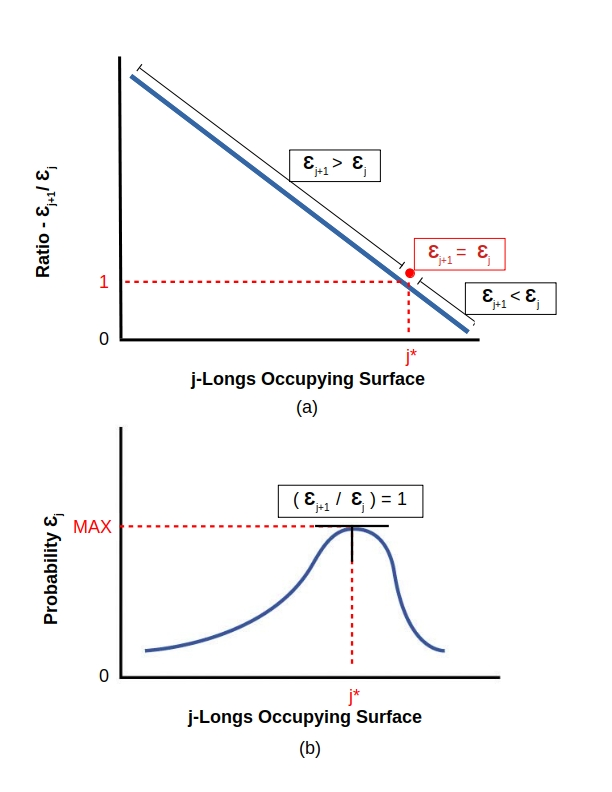
\includegraphics[scale=0.50]{fig9ab.jpg}
\caption{}
\label{figure 9}
\end{figure}

\subsection{Derivation of Boltzmann Entropy from Ratio Approximation}

Initially, we shall take the natural logarithm of our ratio $\frac{|\mathcal{E}_{j+1}|}{|\mathcal{E}_{j}|}$. Then we proceed to expand the expression using known logarithmic properties and multiply the whole expression by the Boltzmann Constant.
\begin{eqnarray*}
k_B\cdot \log\left(\frac{|\mathcal{E}_{j+1}|}{|\mathcal{E}_{j}|}\right)  & = & 
k_B\cdot\left(\log\left|\mathcal{E}_{j+1}\right|-\log\left|\mathcal{E}_{j}\right|\right)  \\
&= & \left(k_B\cdot \log\left|\mathcal{E}_{j+1}\right|\right)-\left(k_B\cdot \log\left|\mathcal{E}_{j}\right|\right)
\end{eqnarray*}

\noindent This is evidently just the difference of Boltzman entropies of $j$ and $j+1$,

$$ =\; S_{j+1}-S_{j}\;=\; \Delta S_{j\to j+1} \,.$$




%\bibliography{LongShort}

\end{document}